% packages and themes
\documentclass{beamer}

\mode<presentation> {
\usetheme{Madrid}
\usecolortheme{dolphin}

}
\usepackage[normalem]{ulem}
\usepackage{inconsolata}

\usepackage{graphicx} % Allows including images
\usepackage{booktabs} % Allows the use of \toprule, \midrule and \bottomrule in tables
\usepackage{outlines}
\usepackage[gen]{eurosym}

\title[]{Open Science in Statistics \& Machine Learning\newline Winter 2022} 

\author{Benedikt Arnthof} 
\institute[LMU München] 
{
Code Sharing in Python Using pipenv\\
\& 
\\
Reproducing Code Sharing in R Using rdocker/dockr
 \\ 
\medskip 
}
\date{\today} % Date, can be changed to a custom date

\begin{document}

\begin{frame}
\titlepage 
\end{frame}

\begin{frame}
\frametitle{Overview}

Part One: Code Sharing in Python Using pipenv 
\begin{itemize}
    \item The Task at Hand
    \item Google Colab
    \item pipenv
    \item Versioning with pipenv
\end{itemize}
\medskip
Part Two: Code Sharing in R Using rocker/dockr
\begin{itemize}
    \item Results \& Comments
\end{itemize}
\medskip
Part Three: Discussion
\end{frame}

\section{Code Sharing in Python Using pipenv} 

\subsection{The Task at Hand}
\begin{frame}
\frametitle{Code Sharing in Python Using pipenv}
\framesubtitle{The Task at Hand}
\begin{itemize}
    \item We propose a new, ground-breaking image augmentation technique!
    \item We implemented it using the Albumentations (Buslaev et al., 2020) package
    \item We train models (CNNs) on MNIST (LeCun et al., 1998) with PyTorch (Paszke et al., 2019)
    \item We present two different versions of our code (One deprecated, one updated)
    \item We manage dependencies using pipenv \& make our results 100\% reproducible
\end{itemize}
\vspace{1cm}
How did we tackle all this?\\
With Colab!
\end{frame}

\begin{frame}
\frametitle{Code Sharing in Python Using pipenv}
\framesubtitle{What is Colab?}
\begin{itemize}
    \item Colaboratory (Colab) is a product from Google Research
    \item It is a hosted Jupyter notebook service that requires \textbf{no setup}
    \item Also allows you to access GPUs (for a limited amount of time)
    \item BASH commands can be executed with the \textbf{!} operator
    \item Does come with limitations: No file sharing, crypto-mining, deepfakes etc.
\end{itemize}
\end{frame}


\section{Code Sharing in Python Using pipenv}
\begin{frame}
\frametitle{Code Sharing in Python Using pipenv}
\framesubtitle{What is pipenv?}
A project by Kenneth Reitz to avoid problems with \textbf{requirements.txt}
\medskip
\begin{itemize}
    \item As different versions of sub-dependencies are released, the result of a fresh \texttt{\$ pip install -r requirements.txt}  will result in different packages being installed, and potentially, your application failing for unknown and hidden reasons.
    \item If exact requirements, including sub-dependencies are listed with \texttt{\$ pip freeze} we still have to find a way to keep track of individual package updates and keep everything under versioning. This can get very tedious in large projects.
\end{itemize}
\medskip
\footnotesize
https://kennethreitz.org/essays/2016/02/25/a-better-pip-workflow
\end{frame}

\begin{frame}
\frametitle{Code Sharing in Python Using pipenv}
\framesubtitle{Colab pipenv Setup \& Workflow}
To use pipenv in Colab we have to do a tiny bit of hacking!
\begin{itemize}
    \item \texttt{!pip install --user pipenv}
    \item \texttt{\# add the location of the pipenv scripts to \$PATH\\
    import os\\
    os.environ['PATH'] += ':/root/.local/bin'}
\end{itemize}
After this we can start installing packages to our virtual environment: 
\begin{itemize}
    \item \texttt{!pipenv install albumentations\\
    !pipenv install torch~=1.12\\
    !pipenv install torchvision==0.13.0}
    \item \texttt{!pipenv graph}
\end{itemize}
To mirror the setup of our project on Github we simply run:
\begin{itemize}
    \item \texttt{!pipenv install}
\end{itemize}
In the root directory of the repo after cloning.
\end{frame}

\begin{frame}
\frametitle{Code Sharing in Python Using pipenv}
\framesubtitle{Project Structure}
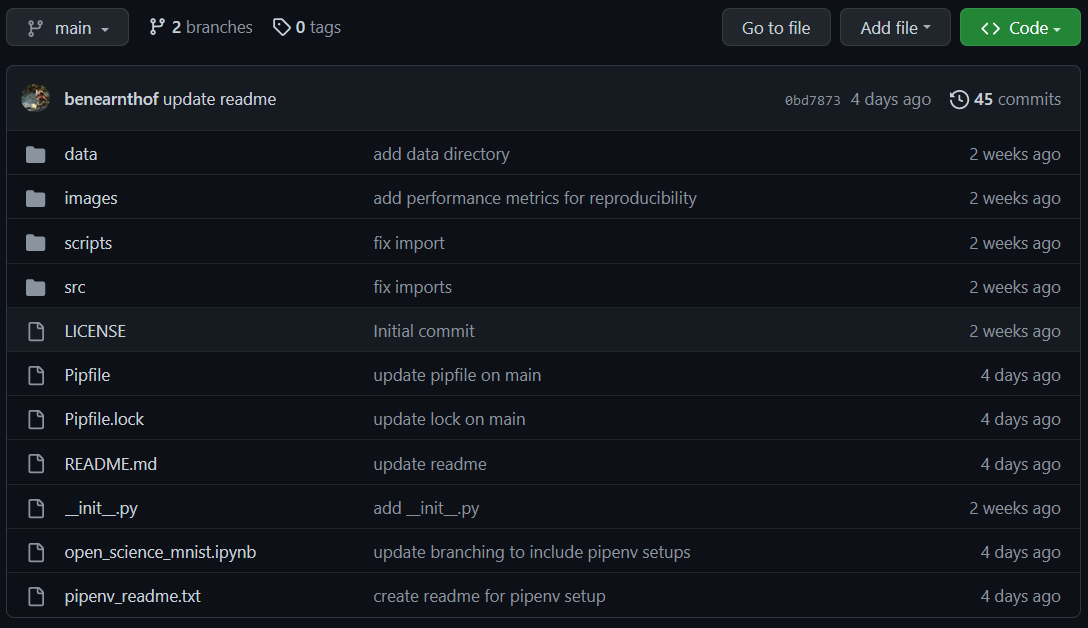
\includegraphics[width=0.9\columnwidth]{/images/repo.PNG}\\
Root directory of the project repo.
\end{frame}

\begin{frame}
\frametitle{Code Sharing in Python Using pipenv}
\framesubtitle{Keeping it Simple}
How do we add data augmentation to MNIST without confusing potential users?\\
\medskip
Two requirements:\\
\medskip
\begin{itemize}
    \item Extending the MNIST dataset class with our own \texttt{\_\_getitem\_\_} method 
    \item Adding our own \texttt{DataLoader} subclasses that initialize with our custom dataset
\end{itemize}
\medskip
The transformations can then simply be composed from basic Albumentation transforms \& passed to our \texttt{DataLoader}
\end{frame}

\subsection{Code Sharing in Python Using pipenv}
\begin{frame}
\frametitle{Code Sharing in Python Using pipenv}
\framesubtitle{A quick glance at our models}
Since we're analysing images with one colour channel we used simple 2D CNNs for our experiments: 
\begin{itemize}
    \item Two Convolutional layers, two Dropout layers, \& two Linear layers
    \item With ReLU activations after the first Conv and Linear layer respectively
    \item And 2D Max-Pooling after the second Conv layer
\end{itemize}
Two versions of this model were trained; one with, and one without augmenting the data.
\end{frame}


\subsection{Results}
\begin{frame}
\frametitle{Code Sharing in Python Using pipenv}
\framesubtitle{Results}
After training both of our models for 10 epochs on the training set we obtain the following test performances:\\
\medskip
\textbf{Basic Model:}
\begin{itemize}
    \item Overall Test Accuracy: \textbf{98.7\%}
    \item Worst Single Class Performance: \textbf{96.3\%} for class \textbf{9}
\end{itemize}
\textbf{Augmented Model:}
\begin{itemize}
    \item Overall Test Accuracy: \textbf{96.6\%}
    \item Worst Single Class Performance: \textbf{94.3\%} for class \textbf{9}
\end{itemize}
Our augmentation technique seems to degrade performance.\\ Can we make a guess why that might be?
\end{frame}

\subsection{Versioning}
\begin{frame}
\frametitle{Code Sharing in Python Using pipenv}
\framesubtitle{Versioning with pipenv}
Let's say we want to update our code to avoid using the deprecated \texttt{dropout2d}.\\
\medskip
How do we keep our virtualenv intact \& avoid deleting old code?
\medskip
By \textbf{Branching!}
\begin{itemize}
    \item \texttt{!git pull} \# pull fresh branches from The Hub
    \item \texttt{!git checkout update\_models} \# checkout the relevant branch
    \item \texttt{!git status} \# mitigate paranoia
\end{itemize}
After we obtained the updated code and the respective Pipfile \& Pipfile.lock files we can create a fresh pipenv:
\begin{itemize}
    \item \texttt{!pip install --user pipenv}
    \item \texttt{!pipenv install}
\end{itemize}
\end{frame}

\subsection{Reproducibility}
\begin{frame}
\frametitle{Code Sharing in Python Using pipenv}
\framesubtitle{Ensuring Reproducibility}
To ensure Reproducibility we have to set three different random seeds:
\medskip
\begin{itemize}
    \item The Python internal \texttt{random} seed
    \item The Numpy random seed for our Augmentations
    \item The Torch random seed for initialization \& training
\end{itemize}
\medskip
Can we think of anything else that may cause issues with reproducibility?
\end{frame}

\section{Appendix}
\begin{frame}
\frametitle{Code Sharing in Python Using pipenv}
\framesubtitle{Ensuring Reproducibility with Distributed Training}
Loading data to multiple devices (GPUs) in parallel may not be deterministic. Use \\
\begin{itemize}
    \item \texttt{worker\_init\_fn()} and \texttt{generator}
\end{itemize}
to preserve reproducibility.\\
\medskip
Training CNNs on CUDA devices may be non-deterministic. Use\\
\begin{itemize}
    \item \texttt{torch.backends.cudnn.deterministic = True} or 
    \item \texttt{torch.use\_deterministic\_algorithms(True)}
\end{itemize}
to preserve reproducibility.\\
\medskip
RNNs and LSTMs may also have non-deterministic behavior. Refer to the pytorch docs for more details.\\
\medskip
\footnotesize
https://pytorch.org/docs/stable/notes/randomness.html
\end{frame}

\begin{frame}
\frametitle{Code Sharing in Python Using pipenv}
\framesubtitle{Serving Data \& Models}
We are very fortunate that MNIST has become the de facto standard dataset in ML.\\
How would you serve data to ensure reproducibility?\\
\medskip
Training (even on CPU only) of our models is very quick! how could we package, or even serve, models for inference and performance testing?
\medskip
What should be added to the repository if the project keeps growing?
\end{frame}

\section{Reproducing Project 9}
\begin{frame}
\frametitle{Code Sharing in R Using rocker/dockr}
\framesubtitle{Reproducing Results}
Analysis:
\begin{itemize}
    \item Ran out of the box 
    \item Exact package versions were found in Dockerfile
\end{itemize}
\medskip
Docker: 
\begin{itemize}
    \item Issues (on my end) with Docker Desktop (Windows).
    \item Using WSL and/or Ubuntu 20 solved the problems
    \item Only one typo in: \texttt{docker run -v ~/your\_prefered\_directory\_here/docker\_results:home/results mushroom\_classification} needed to be swapped with \texttt{mushroom\_analysis} 
\end{itemize}
\end{frame}


\begin{frame}{Sources}
Pytorch:
\begin{itemize}
    \item \tiny https://arxiv.org/abs/1912.01703
    \item \tiny https://pytorch.org/docs/stable/notes/randomness.html\\
\end{itemize}
Albumentations:
\begin{itemize}
    \item \tiny https://albumentations.ai/\\
    \item \tiny https://www.mdpi.com/2078-2489/11/2/125\\
\end{itemize}
Pipenv:
\begin{itemize}
    \item \tiny https://pipenv.pypa.io/en/latest/
    \item \tiny https://kennethreitz.org/essays/2016/02/25/a-better-pip-workflow
\end{itemize}
MNIST:
\begin{itemize}
    \item \tiny http://yann.lecun.com/exdb/mnist/
    \item \tiny https://pytorch.org/vision/stable/generated/torchvision.datasets.MNIST.html
    \item \tiny https://pytorch.org/vision/stable/\_modules/torchvision/datasets/mnist.html\#MNIST
\end{itemize}



\end{frame}

\end{document}
